\subsubsection{Simple convection in a quarter of a 2d annulus}
\label{sec:shell-simple-2d}

Let us start this sequence of cookbooks using a simpler situation: convection in
a quarter of a 2d shell. We choose this setup because 2d domains allow for much
faster computations (in turn allowing for more experimentation) and because
using a quarter of a shell avoids a pitfall with boundary conditions we will
discuss in the next section. Because it's simpler to explain what we want to
describe in pictures than in words, Fig.~\ref{fig:simple-shell-2d} shows the
domain and the temperature field at a few time steps. In addition, you can find
a movie of how the temperature evolves over this time period at
\url{http://www.youtube.com/watch?v=d4AS1FmdarU}.%
\footnote{In YouTube, click on the gear symbol at the bottom right of the
player window to select the highest resolution to see all the details of this
video.}

\begin{figure}[tb]
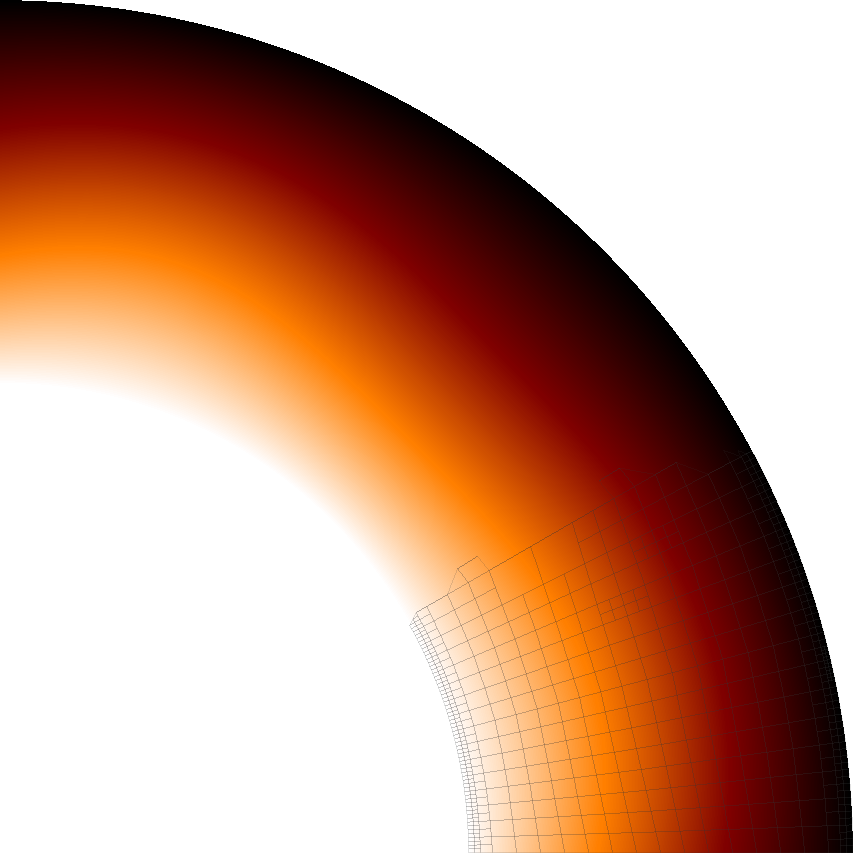
\includegraphics[width=0.32\textwidth]{x-movie0000.png}
\hfill
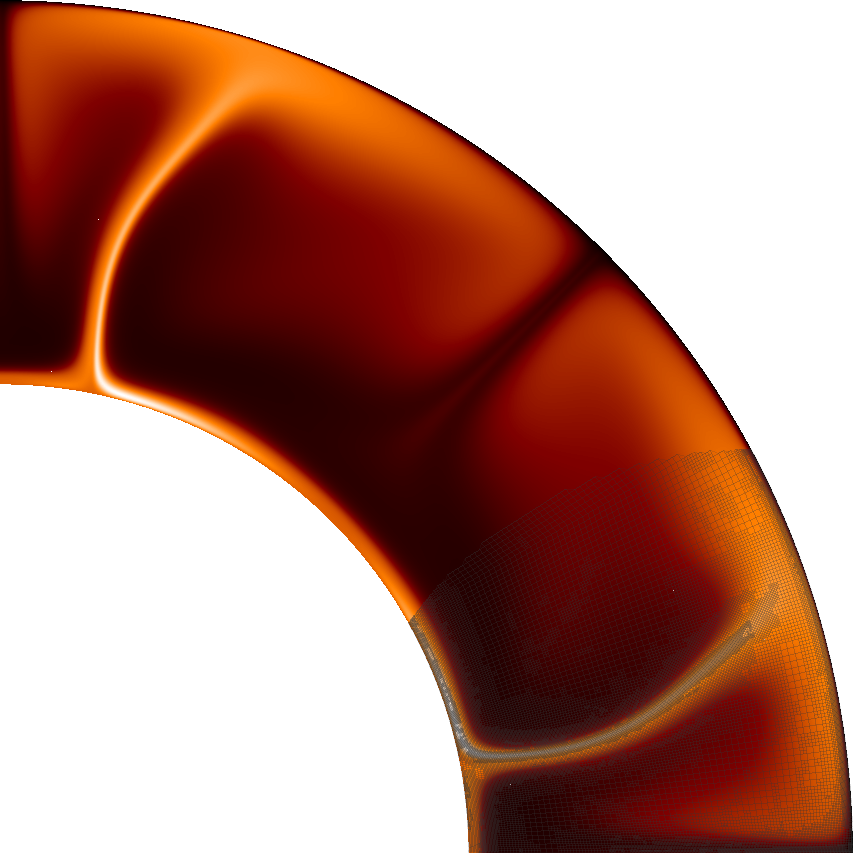
\includegraphics[width=0.32\textwidth]{x-movie0008.png}
\hfill
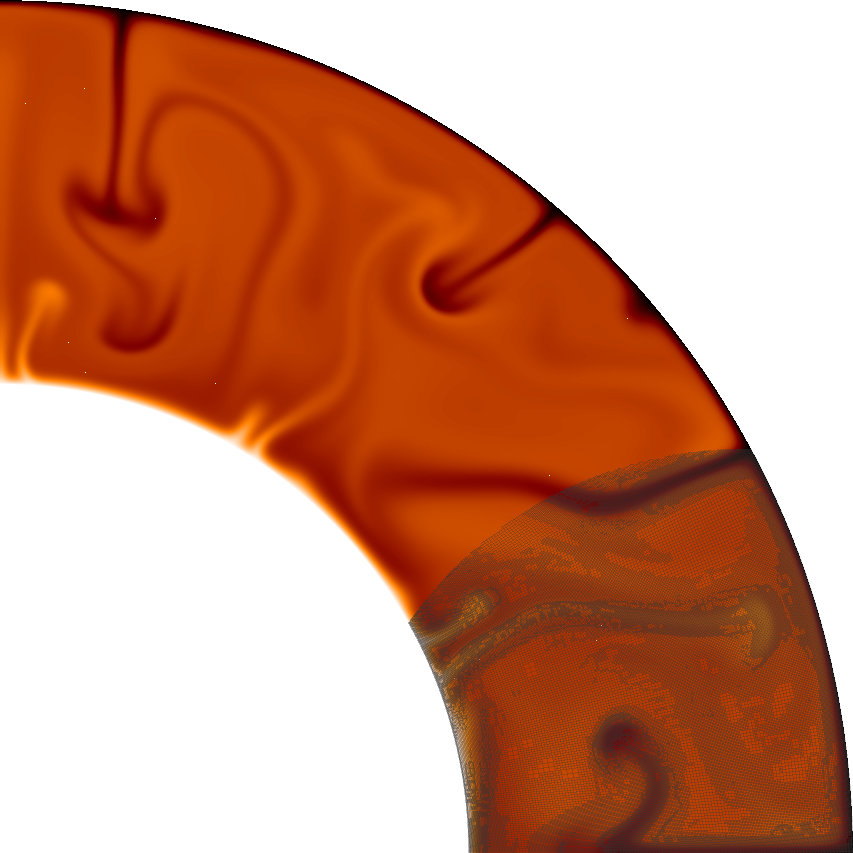
\includegraphics[width=0.32\textwidth]{x-movie1000.png}
\caption{\it Simple convection in a quarter of an annulus: Snapshots of the
temperature field at times $t=0$, $t=\num{1.2e7}$ years (time step 2135), and
$t=10^9$ years (time step 25,662). The bottom right part of each figure shows an
overlay of the mesh used during that time step.}
\label{fig:simple-shell-2d}
\end{figure}

Let us just start by showing the input file (which you can find in
\url{cookbooks/shell_simple_2d/shell_simple_2d.prm}):

\lstinputlisting[language=prmfile]{shell.prm.out}

In the following, let us pick apart this input file:
\begin{enumerate}
  \item Lines 1--4 are just global parameters. Since we are interested in
  geophysically realistic simulations, we will use material parameters that
  lead to flows so slow that we need to measure time in years, and we will set
  the end time to 1.5 billion years -- enough to see a significant amount of
  motion.

  \item The next block (lines 7--14) describes the material that is convecting
  (for historical reasons, the remainder of the parameters that describe the
  equations is in a different section, see the fourth point below). We choose
  the simplest material model \aspect{} has to offer where the viscosity is
  constant (here, we set it to $\eta=10^{22} \si{Pa .  s}$) and so are
  all other parameters except for the density which we choose to be
  $\rho(T)=\rho_0(1-\alpha (T-T_{\text{ref}}))$ with $\rho_0=3300
  \si{kg}\;\si{m}^{-3}$, $\alpha=\num{4e-5} \si{K}^{-1}$ and
  $T_{\text{ref}}=293 \si{K}$. The remaining material parameters remain at their
  default values and you can find their values described in the documentation of
  the \texttt{simple} material model in
  Sections~\ref{parameters:Material_20model} and
  \ref{parameters:Material_20model/Simple_20model}.

  \item Lines 17--25 then describe the geometry. In this simple case, we will
  take a quarter of a 2d shell (recall that the dimension had previously been
  set as a global parameter) with inner and outer radii matching those of a
  spherical approximation of Earth.

  \item The second part of the model description and boundary values follows in
  lines 28--42. The boundary conditions require us to look up how the geometry model
  we chose (the \texttt{spherical shell} model) assigns boundary indicators to
  the four sides of the domain. This is described in
  Section~\ref{parameters:Geometry_20model} where the model announces that
  boundary indicator zero is the inner boundary of the domain, boundary
  indicator one is the outer boundary, and the left and right boundaries for a
  2d model with opening angle of 90 degrees as chosen here get boundary
  indicators 2 and 3, respectively. In other words, the settings in the input
  file correspond to a zero velocity at the inner boundary and tangential flow
  at all other boundaries. We know that this is not realistic at the bottom, but
  for now there are of course many other parts of the model that are not
  realistic either and that we will have to address in subsequent cookbooks.
  Furthermore, the temperature is fixed at the inner and outer boundaries (with
  the left and right boundaries then chosen so that no heat flows across them,
  emulating symmetry boundary conditions) and, further down, set to values of
  700 and 4000 degrees Celsius -- roughly realistic for the bottom of the crust
  and the core-mantle boundary.

  \item Lines 45--47 describe that we want a model where equation
  \eqref{eq:temperature} contains the shear heating term $2\eta
  \varepsilon(\mathbf u):\varepsilon(\mathbf u)$ (noting that the default is to
  use an incompressible model for which the term $\frac{1}{3}(\nabla \cdot
  \mathbf u)\mathbf 1$ in the shear heating contribution is zero). Considering a
  reasonable choice of heating terms is not the focus of this simple cookbook,
  therefore we will leave a discussion of possible and reasonable heating terms
  to another cookbook.

  \item The description of what we want to model is complete by specifying
  that the initial temperature is a perturbation with hexagonal symmetry from a
  linear interpolation between inner and outer temperatures (see
  Section~\ref{parameters:Initial_20composition_20model}), and what kind of gravity model
  we want to choose (one reminiscent of the one inside the Earth mantle, see
  Section~\ref{parameters:Gravity_20model}).

  \item The remainder of the input file consists of a description of how to
  choose the initial mesh and how to adapt it (lines 60--65) and what to do at
  the end of each time step with the solution that \aspect{} computes for us (lines 68--81).
  Here, we ask for a variety of statistical quantities and for graphical output
  in VTU format every million years.
\end{enumerate}

\note{Having described everything to \aspect{}, you may want to view the video linked
to above again and compare what you see with what you expect. In fact, this is
what one should always do having just run a model: compare it with expectations to make
sure that we have not overlooked anything when setting up the model or that
the code has produced something that doesn't match what we thought we should
get. Any such mismatch between expectation and observed result is typically a
learning opportunity: it either points to a bug in our input file, or it
provides us with insight about an aspect of reality that we had not foreseen.
Either way, accepting results uncritically is, more often than not, a way to
scientifically invalid results.}

The model we have chosen has a number of inadequacies that
make it not very realistic (some of those happened more as an accident while
playing with the input file and weren't a purposeful experiment, but we left
them in because they make for good examples to discuss below).
Let us discuss these issues in the following.

\paragraph{Dimension.} This is a cheap shot but it is nevertheless true that the
world is three-dimensional whereas the simulation here is 2d. We will address
this in the next section.

\paragraph{Incompressibility, adiabaticity and the initial conditions.} This one
requires a bit more discussion. In the model selected above, we have chosen a
model that is incompressible in the sense that the density does not depend on
the pressure and only very slightly depends on the temperature.
In such models, material that rises up does not cool down due to
expansion resulting from the pressure dropping, and material that is transported
down does not adiabatically heat up. Consequently, the adiabatic temperature
profile would be constant with depth, and a well-mixed model with hot inner and
cold outer boundary would have a constant temperature with thin boundary layers
at the bottom and top of the mantle. In contrast to this, our initial
temperature field was a perturbation of a linear temperature profile.

There are multiple implications of this. First, the temperature difference
between outer and inner boundary of 3300 K we have chosen in the input file is
much too large. The temperature difference that drives the convection,
is the difference \textit{in addition} to the temperature increase a volume of
material would experience if it were to be
transported adiabatically from the surface to the core-mantle boundary. This
difference is much smaller than 3300 K in reality, and we can expect convection
to be significantly less vigorous than in the simulation here. Indeed, using
the values in the input file shown above, we can compute the Rayleigh number for
the current case to be%
\footnote{Note that the density in 2d has units $\si{kg}\,\si{m}^{-2}$}
\begin{equation*}
  \textrm{Ra}
  =
  \frac{g\, \alpha  \Delta T  \rho  L^3}{\kappa\eta}
=
  \frac{10\, \si{m}\,\si{s}^{-2} \times \num{4e-5}\, \si{K}^{-1} \times 3300\,
  \si{K} \times 3300\, \si{kg}\,\si{m}^{-3} \times (\num{2.86e6}
  \, \si{m})^3}{10^{-6}\, \si{m}^2\,\si{s}^{-1}\times 10^{22}\,
  \si{kg}\,\si{m}^{-1}\,\si{s}^{-1}}.
\end{equation*}

Second, the initial temperature profile we chose is not realistic -- in fact, it
is a completely unstable one: there is hot material underlying cold one, and
this is not just the result of boundary layers. Consequently, what happens in
the simulation is that we first overturn the entire temperature field with the
hot material in the lower half of the domain swapping places with the colder
material in the top, to achieve a stable layering except for the boundary
layers. After this, hot blobs rise from the bottom boundary layer into the cold
layer at the bottom of the mantle, and cold blobs sink from the top, but their
motion is impeded about half-way through the mantle once they reach material
that has roughly the same temperature as the plume material. This impedes
convection until we reach a state where these plumes have sufficiently mixed the
mantle to achieve a roughly constant temperature profile.

This effect is visible in the movie linked to above where convection does not
penetrate the entire depth of the mantle for the first 20 seconds
(corresponding to roughly the first 800 million years). We can also see this
effect by plotting the root mean square velocity, see the left panel of
Fig.~\ref{fig:simple-shell-2d-rms}. There, we can see how the average velocity
picks up once the stable layering of material that resulted from the initial
overturning has been mixed sufficiently to allow plumes to rise or sink through
the entire depth of the mantle.

\begin{figure}[tb]
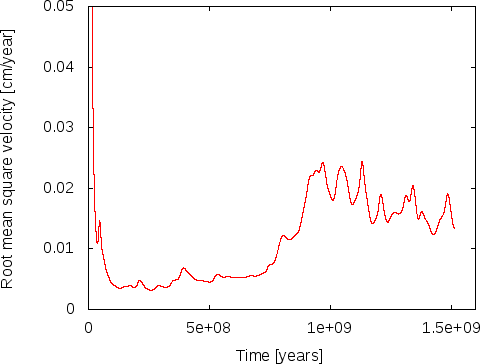
\includegraphics[width=0.48\textwidth]{rms.png}
\hfill
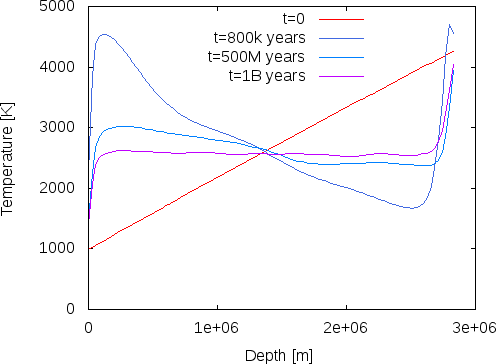
\includegraphics[width=0.48\textwidth]{depth_average_temperature.png}
\caption{\it Simple convection in a quarter of an annulus. Left: Root mean
square values of the velocity field. The initial spike (off the scale) is due to
the overturning of the unstable layering of the temperature. Convection is suppressed for the
first 800 million years due to the stable layering that results from it. The
maximal velocity encountered follows generally the same trend and is in the
range of 2--3 cm/year between 100 and 800 million years, and 4--8 cm/year
following that. Right: Average temperature at various depths for $t=0$,
$t=800,000$ years, $t=\num{5e8}$ years, and $t=10^9$ years.}
\label{fig:simple-shell-2d-rms}
\end{figure}

The right panel of Fig.~\ref{fig:simple-shell-2d-rms} shows a different way of
visualizing this, using the average temperature at various depths of the model
(this is what the \texttt{depth average} postprocessor computes). The figure
shows how the initially linear unstable layering almost immediately reverts
completely, and then slowly equilibrates towards a temperature profile that is
constant throughout the mantle (which in the incompressible model chosen here
equates to an adiabatic layering) except for the boundary layers at the inner
and outer boundaries. (The end points of these temperature profiles do not
exactly match the boundary values specified in the input file because we
average temperatures over shells of finite width.)

A conclusion of this discussion is that if we want to evaluate the statistical
properties of the flow field, e.g., the number of plumes, average velocities or
maximal velocities, then we need to restrict our efforts to times after
approximately 800 million years in this simulation to avoid the effects of our
inappropriately chosen initial conditions. Likewise, we may actually want to
choose initial conditions more like what we see in the model for later times,
i.e., constant in depth with the exception of thin boundary layers, if we want
to stick to incompressible models.

\paragraph{Material model.}
The model we use here involves viscosity, density, and thermal property
functions that do not depend on the pressure, and only the density varies
(slightly) with the temperature. We know that this is not the case in nature.

\paragraph{Shear heating.}
When we set up the input file, we started with a model that includes the
shear heating term $2\eta \varepsilon(\mathbf u):\varepsilon(\mathbf u)$ in
eq.~\eqref{eq:temperature}. In hindsight, this may have been the wrong decision,
but it provides an opportunity to investigate whether we think that the results of our
computations can possibly be correct.

We first realized the issue when looking at the heat flux that the
\texttt{heat flux statistics} postprocessor computes. This is shown in the left
panel of Fig.~\ref{fig:simple-shell-2d-heatflux}.%
\footnote{The \texttt{heat flux statistics} postprocessor computes heat fluxes
through parts of the boundary in \textit{outward} direction, i.e., from the
mantle to the air and to the core. However, we are typically interested in the
flux from the core into the mantle, so the figure plots the negative of the
computed quantity.}
There are two issues one should notice here.
The more obvious one is that the flux from the mantle to the air is consistently
higher than the heat flux from core to mantle. Since we have no radiogenic
heating model selected (see the \texttt{List of model names}
\index[prmindex]{List of model names}
\index[prmindexfull]{Heating model!List of model names}
parameter in the \texttt{Heating model} section of the input file; see also
Section~\ref{parameters:Heating_20model}), in the long run the heat output
of the mantle must equal the input, unless is cools. Our misconception was that
after the 800 million year transition, we believed that we had reached a steady
state where the average temperature remains constant and convection simply
moves heat from the core-mantle boundary the surface. One could also be tempted
to believe this from the right panel in Fig.~\ref{fig:simple-shell-2d-rms} where
it looks like the average temperature does at least not change dramatically.
But, it is easy to convince oneself that that is not the case: the
\texttt{temperature statistics} postprocessor we had previously selected also
outputs data about the mean temperature in the model, and it looks like shown in
the left panel of Fig.~\ref{fig:simple-shell-2d-temperature}. Indeed, the
average temperature drops over the course of the 1.2 billion years shown here.
We could now convince ourselves that indeed the loss of thermal
energy in the mantle due to the drop in average temperature is exactly what
fuels the persistently imbalanced energy outflow. In essence, what this would
show is that if we kept the temperature at the boundaries constant, we would
have chosen a mantle that was initially too hot on average to be sustained by
the boundary values and that will cool until it will be in energetic balance and
on longer time scales, in- and outflow of thermal energy would balance each
other.


\begin{figure}[tb]
  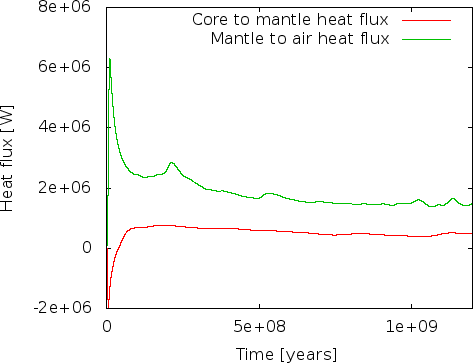
\includegraphics[width=.48\textwidth]{heat-flux.png}
  \hfill
  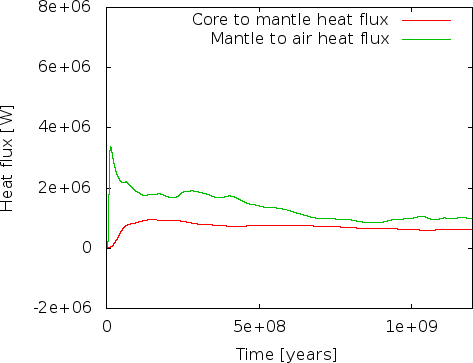
\includegraphics[width=0.48\textwidth]{heat-flux-noshear.png}
  \caption{\it Simple convection in a quarter of an annulus. Left: Heat flux
  through the core-mantle and mantle-air boundaries of the domain for the
  model with shear heating. Right: Same for a model without shear heating.}
  \label{fig:simple-shell-2d-heatflux}
\end{figure}


\begin{figure}[tb]
  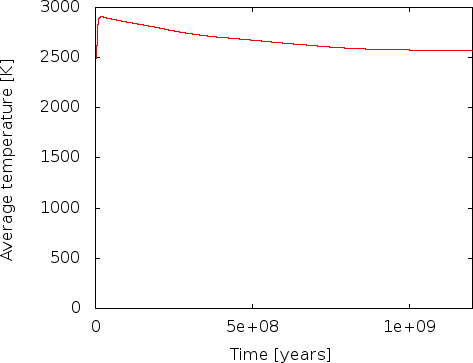
\includegraphics[width=.48\textwidth]{avg-temperature.png}
  \hfill
  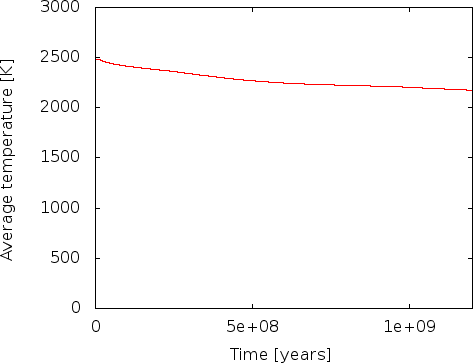
\includegraphics[width=0.48\textwidth]{avg-temperature-noshear.png}
  \caption{\it Simple convection in a quarter of an annulus. Left: Average
  temperature throughout the model for the
  model with shear heating. Right: Same for a model without shear heating.}
  \label{fig:simple-shell-2d-temperature}
\end{figure}

However, there is a bigger problem. Fig.~\ref{fig:simple-shell-2d-heatflux}
shows that at the very beginning, there is a spike in energy flux through the
outer boundary. We can explain this away with the imbalanced initial temperature
field that leads to an overturning and, thus, a lot of hot material rising close
to the surface that will then lead to a high energy flux towards the cold upper
boundary. But, worse, there is initially a \textit{negative} heat flux into the
mantle from the core -- in other words, the mantle is \textit{losing} energy to
the core. How is this possible? After all, the hottest part of the mantle in our
initial temperature field is at the core-mantle boundary, no thermal energy
should be flowing from the colder overlying material towards the hotter material
at the boundary! A glimpse of the solution can be found in looking at the
average temperature in Fig.~\ref{fig:simple-shell-2d-temperature}: At the
beginning, the average temperature \textit{rises}, and apparently there are
parts of the mantle that become hotter than the 4273 K we have given the core,
leading to a downward heat flux. This heating can of course only come from the
shear heating term we have accidentally left in the model: at the beginning, the
unstable layering leads to very large velocities, and large velocities lead to
large velocity gradients that in turn lead to a lot of shear heating! Once the
initial overturning has subsided, after say 100 million years (see the mean
velocity in Fig.~\ref{fig:simple-shell-2d-rms}), the shear heating becomes
largely irrelevant and the cooling of the mantle indeed begins.

Whether this is really the case is of course easily verified: The right panels
of Figs.~\ref{fig:simple-shell-2d-heatflux}
and \ref{fig:simple-shell-2d-temperature} show heat fluxes and average
temperatures for a model where we have switched off the shear heating by setting

\lstinputlisting[language=prmfile]{shearheat.part.prm.out}

Indeed, doing so leads to a model where the heat flux from core to mantle is
always positive, and where the average temperature strictly drops!


\paragraph{Summary.} As mentioned, we will address some of the issues we have
identified as unrealistic in the following sections.
However, despite all of this, some things are at least at the right order of
magnitude, confirming that what \aspect{} is computing is reasonable. For
example, the maximal velocities encountered in our model (after the 800 million
year boundary) are in the range of 6--7cm per year, with occasional excursions
up to 11cm. Clearly, something is going in the right direction.



